\documentclass{article}

\usepackage[margin=3cm]{geometry}
\usepackage{amsmath}
\usepackage{amssymb}
\usepackage{tikz}
\usepackage{listings}
\lstset{
    basicstyle=\scriptsize,
    numbers=left,
    numbersep=5pt
}

\title{\Large\bfseries CS 477: Formal Software Development Methods \\
Fall 2016 \\
Homework 3}
\author{Chiao Hsieh, chsieh16@illinois.edu}

\begin{document}
\maketitle

\begin{enumerate}
\item \textbf{[30 points]}

This exercise is regarding a real bug, the \textit{Zune bug},
caused by a piece of code in Microsoft's Zune player,
which takes an integer representing days and finds the corresponding year.

Find the bug using Dafny (see attached file zune.dfy).
And fix the code (if you use any source on the internet,
you must cite the source).
And prove that the code terminates using Dafny.

Note: The IsLeapYear() method has not been implemented.
Its implementation is not important for termination.
Submit a hardcopy print-out of your final program and also send your file by email.

\medskip
Ans.
\medskip

\textbf{Bug:} When $days = 366$ and the $year$ is a leap year,
$days$ won't decrease and therefore the loop won't terminate.

\textbf{Fix:}
Since the bug only happen at $days = 366$,
we change the loop condition to $day > 366$,
and do an extra check after the loop.
The same rank function can be used to prove termination.
\lstinputlisting{zune-modified.dfy}

\item \textbf{[20 points]}

Let $(L, \sqsubseteq, \sqcup, \sqcap, 0, 1)$ be a lattice.
Let $f : L \to L$ be a monotonic function.
Let $a \in L$ with $f(a) \sqsubseteq a$.
Prove, formally, that:

\begin{itemize}
    \item For every $n \in \mathbb{N}$, $f^n(a)\sqsubseteq a$
    \item Assume that $p$ is a fixed point of $f$,
          and also assume that $f^m(a) = f^{m+1}(a) = r$,
          for a particular $m \in \mathbb{N}$.
          Then prove that $p \sqsubseteq a$ implies $p \sqsubseteq r$.
\end{itemize}

\medskip
Ans.
\medskip


We can prove $f^n(a)\sqsubseteq a$ for all $n \in \mathbb{N}$ by induction on $n$.

\textbf{Base case}: $n = 1$

$f(a) \sqsubseteq a$ trivially holds.

\textbf{Induction}: Assume that $f^{n-1}(a) \sqsubseteq a$

By definition of monotonicity that $x \sqsubseteq y \to f(x) \sqsubseteq f(y)$,
we know $f(f^{n-1}(a)) \sqsubseteq f(a) \sqsubseteq a$.

Hence, $f^n(a) \sqsubseteq a$ holds for all $n \in \mathbb{N}$

Next we prove $p \sqsubseteq a$ implies $p \sqsubseteq r$.
Because $f$ is monotonic,
we know that $f^m(p) \sqsubseteq f^m(a)$ when $p \sqsubseteq a$.
Since $p$ is a fixed point, that is, $f(p) = p$,
we can derive that $p \sqsubseteq f^m(a) = r$. 

\item \textbf{[30 points]}

We are exploring predicate abstraction in this exercise. \\
Assume a program has a single variable $x$. \\
Assume we track three predicates:\\
$p_1$: true iff $x$ is multiple of 8\\
$p_2$: true iff $x$ is multiple of 2\\
$p_3$: true iff $x = 0$

Describe accurate abstract transformers for the following operation:
\begin{itemize}
    \item \verb|x:=c;| (where \verb|c| is a constant)
    \item \verb|x:=2*x;|
    \item \verb|x:=4*x;|
\end{itemize}

For each of the statements above, you need to give a sequence of statements that
update the value of $p_1$,$p_2$,$p_3$ that best reflect the effect of the
concrete semantics of the above statements.

Finally, analyze the following program by describing the value of the predicates
after each of these statements, and argue what we can know from the abstract
analysis after the end of the following program:
\begin{verbatim}
    x:=1;
    x:=2*x;
    x:=4*x;
    x:=2*x;
\end{verbatim}

\medskip
Ans.
\medskip

\textbf{Statement} \verb|x:=c|, \\
Since $c$ is constant, it can be further analyzed when translating to Boolean program

when $c$ is odd, \\
\verb|p1 := false; p2 := false; p3 := false;|

when $c$ is $0$,\\
\verb|p1 := true; p2 := true; p3 := true;|

when $c = 2*k$ or $c = 4*k$ where $k$ is odd, \\
\verb|p1 := false; p2 := true; p3 := false;|

else when $c$ must be multiple of 8 but not 0, \\
\verb|p1 := true; p2 := true; p3 := false;|

\bigskip
\textbf{Statement} \verb|x:=2*x|,
\begin{verbatim}
if(!p2)     // x is odd
{ p1 := false; p2 := true; p3 := false;} // New x is even but not 0 or 8*k
else if(p3) // x is 0
{ p1 := true; p2 := true; p3 := true;}   // New x is still 0
else if(p1) // x is 8*k but not zero
{ p1 := true; p2 := true; p3 := false;}  // New x is still 8*k but not zero
else        // x is 2*k or 4*k where k is odd
{ p1 := T; p2 := true; p3 := false;}     // Don't know if new x is multiple of 8
\end{verbatim}
where \verb|T| means unknown (top element).

\bigskip
\textbf{Statement} \verb|x:=4*x|,
\begin{verbatim}
if(!p2)     // x is odd
{ p1 := false; p2 := true; p3 := false;} // New x is 4*k but not 0 or 8*k
else if(p3) // x is 0
{ p1 := true; p2 := true; p3 := true;}   // New x is still 0
else if(p1) // x is 8*k but not zero
{ p1 := true; p2 := true; p3 := false;}  // New x is still 8*k but not zero
else        // x is 2*k or 4*k where k is odd
{ p1 := true; p2 := true; p3 := false;}  // New x must be multiple of 8
\end{verbatim}

Following the above translation,
we can derive the value of predicates after each statement as below.
\begin{verbatim}
{p1 = T & p2 = T & p3 = T}
    x:=1;
{p1 = false & p2 = false & p3 = false}
    x:=2*x;
{p1 = false & p2 = true & p3 = false}
    x:=4*x;
{p1 = true  & p2 = true & p3 = false}
    x:=2*x;
{p1 = true  & p2 = true & p3 = false}
\end{verbatim}
From above, we know that the final value of x must be multiple of 8 but not 0;
\item \textbf{[20 points]}

Perform model-checking manually on the following transition system with
propositions $\{p, q, r\}$.
Check which states satisfy the CTL formula $A(pU(EF q))$ on this system by
listing the precise set of states that satisfy its subformulas, inductively.
\begin{center}
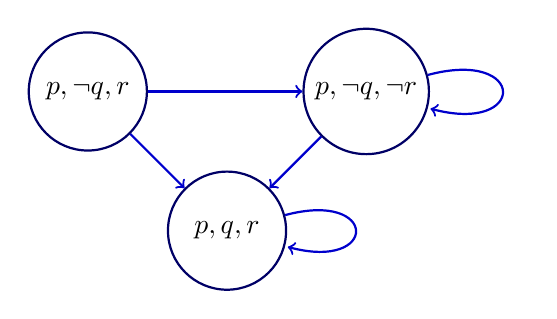
\begin{tikzpicture}[node distance=2.5cm,
roundnode/.style={circle, draw=blue!40!black, thick, minimum size = 15mm},
edge/.style={->, thick, blue!80!black}
]
\node [roundnode] (s2) {$p, q, r$};
\node [roundnode, above right of=s2] (s1) {$p, \neg q, \neg r$};
\node [roundnode, above left of =s2] (s0) {$p, \neg q, r$};

\path (s0) edge [edge] (s1)
      (s0) edge [edge] (s2)
      (s1) edge [edge] (s2)
      (s1) edge [edge, loop right] (s1)
      (s2) edge [edge, loop right] (s2);
\end{tikzpicture}
\end{center}
For every subformula (including the formula itself),
from simper to more complex,
list the precise set of states that satisfy the subformula.

\medskip
Ans.
\medskip

First we list all the sub-formulas, 
$\{p, q, EF q, A(pU(EF q))\}$

\begin{center}
    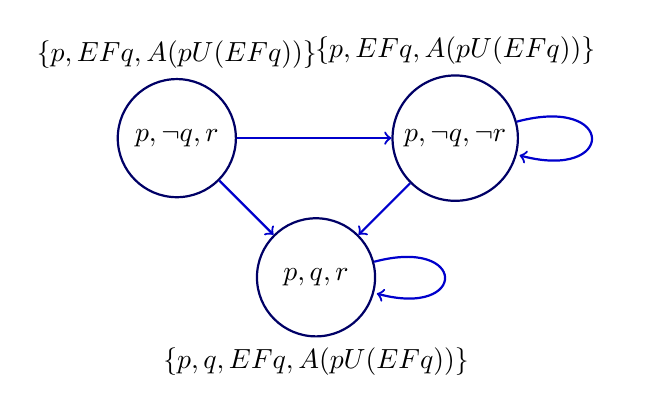
\begin{tikzpicture}[node distance=2.5cm,
    roundnode/.style={circle, draw=blue!40!black, thick, minimum size = 15mm},
    edge/.style={->, thick, blue!80!black}
    ]
    \node [roundnode, label={below:$\{p, q, EF q, A(pU(EF q))\}$}] (s2) {$p, q, r$};
    \node [roundnode, above right of=s2, label={$\{p, EF q, A(pU(EF q))\}$}] (s1) {$p, \neg q, \neg r$};
    \node [roundnode, above left of =s2, label={$\{p, EF q, A(pU(EF q))\}$}] (s0) {$p, \neg q, r$};
    
    \path (s0) edge [edge] (s1)
    (s0) edge [edge] (s2)
    (s1) edge [edge] (s2)
    (s1) edge [edge, loop right] (s1)
    (s2) edge [edge, loop right] (s2);
    \end{tikzpicture}
\end{center}

From above, we conclude that all states satisfy the CTL formula $A(pU(EF q))$.

\end{enumerate}

\end{document}